\documentclass[tikz,border=4pt]{standalone}
\usepackage{pgfplots}
\usepackage{xcolor}
\usepackage[scaled=0.96]{helvet}
\renewcommand{\familydefault}{\sfdefault}
\pgfplotsset{compat=1.18}
\usepgfplotslibrary{groupplots}
\definecolor{PosterBg}{HTML}{EFE2D0}
\definecolor{PosterCard}{HTML}{FCDEB9}
\definecolor{PosterInk}{HTML}{3B3B3B}
\definecolor{PosterAccent}{HTML}{B00300}
\definecolor{PosterGray}{HTML}{5F5F5F}
\definecolor{PosterBorder}{HTML}{CFC3B3}
\definecolor{PosterMuted}{HTML}{E2E2E2}
\definecolor{PosterBlush}{HTML}{F3D5D0}
\pgfplotsset{
  journalaxis/.style={
    axis line style={PosterGray},
    tick style={PosterGray},
    major grid style={draw=PosterBorder},
    ymajorgrids=true,
    xmajorgrids=false,
    xticklabel style={font=\scriptsize, text=PosterInk},
    yticklabel style={font=\scriptsize, text=PosterInk},
    xlabel style={font=\scriptsize, text=PosterInk},
    ylabel style={font=\scriptsize, text=PosterInk},
    title style={font=\scriptsize, align=center, text=PosterInk},
    ticklabel style={text=PosterInk},
    axis background/.style={fill=PosterBg},
  },
  journalbar/.style={
    axis line style={PosterGray},
    tick style={PosterGray},
    major grid style={draw=PosterBorder},
    ymajorgrids=true,
    xticklabel style={font=\small, text=PosterInk},
    yticklabel style={font=\scriptsize, text=PosterInk},
    ylabel style={font=\small, text=PosterInk},
    legend style={draw=none, font=\small, text=PosterInk, /tikz/every even column/.append style={column sep=6pt}},
    ticklabel style={text=PosterInk},
    axis background/.style={fill=PosterBg},
  }
}

\pagecolor{PosterBg}
\begin{document}
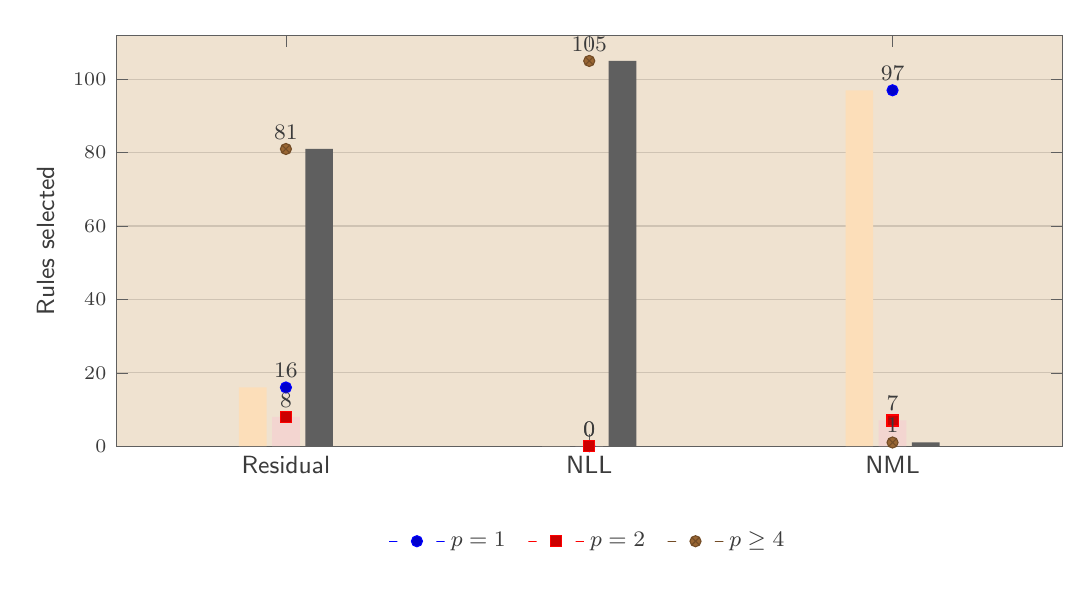
\begin{tikzpicture}
\begin{axis}[
  journalbar,
  width=13.6cm,
  height=6.8cm,
  ymin=0, ymax=112,
  ylabel={Rules selected},
  symbolic x coords={Residual,NLL,NML},
  xtick=data,
  enlarge x limits=0.28,
  nodes near coords,
  every node near coord/.append style={font=\footnotesize, /pgf/number format/precision=0, text=PosterInk},
  legend columns=3,
  legend style={at={(0.5,-0.18)}, anchor=north, font=\footnotesize}
]
\addplot+[ybar, bar width=10pt, bar shift=-12pt, draw=none, fill=PosterCard] coordinates {(Residual,16) (NLL,0) (NML,97)};
\addplot+[ybar, bar width=10pt, bar shift=0pt, draw=none, fill=PosterBlush] coordinates {(Residual,8) (NLL,0) (NML,7)};
\addplot+[ybar, bar width=10pt, bar shift=12pt, draw=none, fill=PosterGray] coordinates {(Residual,81) (NLL,105) (NML,1)};
\legend{$p=1$,$p=2$,$p\ge 4$}
\end{axis}
\end{tikzpicture}
\end{document}
